\part{信息检索与排名}

\textbf{排名}是对象集合组织、排列的方法,反映某种\textbf{规则化需求},而规则化需求的抽象化表达就是\textbf{排名算法}。排名算法思想源于\textbf{信息检索}
(Information Retrieval,IR),历经对图书、专利、网页、图片和音频排名等几个阶段,每个阶段都代表排名算法的一次跨越式发展。

对于一组待排名对象,不同的排名算法所产生的排名结果也不尽相同,影响排名差异性的主要因素是排名算法背后的规则化需求。如果规则化需求明确,如图书管理员要求对所有图书馆中的图书按照价格从高到低重新排列,不同排名算法也能产生相对一致的排名结果(价格相同的图书可能会引发微小差异);如果规则化需求相对模糊,如网络用户希望搜索引擎能够为其提供最相关的搜索结果,由于不同搜索排名算法对需求的解读不尽相同,则可能产生迥然不同的搜索排名结果。明确的规则化需求不仅限定排名算法排名时所依据的标准(或者\textbf{特征、因子}等),甚至还包含具体的\textbf{度量指标},依此作为判断排名精确与否的标准。

在实际应用中,绝大多数的规则化需求相对模糊,对排名算法使用的排名特征和排名精度的度量指标均无约束,从而诞生了各种类型的排名算法。人们试图从不同角度解读规则化需求的确切含义,构造各种约束性的度量指标,并以此为基础,深入研究影响排名度量指标的对象特征,设计出与规则化需求尽量吻合的排名算法及模型。

\chapter{向量空间模型}
在信息检索领域,信息检索系统处理的最基本元素是单词(term)或者中文语境下的词语。通常,系统在执行信息检索之前,会对每篇文档进行分词、索引等基本的预处理工作。在对文档分词以后,可以统计出单词在每篇文档出现的频率,含有此单词的文档集合。系统在检索时会根据检索语句(query)与信息数据库内文档的匹配程度,搜索出相关文档。最原始的信息检索模型是布尔模型(Boolean model),它是一种建立在集合论和布尔代数之上的二元匹配方法。70年代,康奈尔大学
\footnote{\includegraphics[width=2.0mm]{figures/university/cornell.eps}~~~\href{http://www.cornell.edu/}{Cornell University}, 1865}
教授Gerard Salton\footnote{Gerard Salton教授(1927--1995),现代信息检索奠基人,现代搜索技术之父,向量空间模型发明人,主持建立世界上第一个全自动文本处理和检索的实验性开源系统SMART,信息检索领域最高奖项索尔顿奖1983年度首届得主,康奈尔大学计算机系创始人。}
等人\cite{salton1975vector}提出一种“词袋”(bag-of-words)模型,将文档、检索语句表示成数值型的特征向量,再运用代数方法度量检索语句与文档的相似程度,依此对关联文档进行排名。他提出的方法就是至今仍然应用广泛的向量空间模型(Vector Space Model,VSM)。向量空间模型对后续信息检索模型的发展有深远的影响,本节我们开始介绍向量空间模型的基本思想和相关扩展模型。

信息检索是一套复杂的、也是具有层次性的系统。为了方便表示,我们对信息检索系统自顶向下统一建立一套标记。假设系统信息数据库$D$含有$N$篇文档(document),数据文档记作$d$,则数据库可以写作:
\[
    D = \{d_1, d_2, \ldots, d_N\}.
\]
对所有文档分词后,我们就可以创建文档与单词之间的量化特征表示。对于任意一个文档$d\in D$,其数值特征向量可以表示如下:
\[
    V_d = (\omega_1, \omega_2, \ldots, \omega_m)^T\in \mathbb R^m,
\]
其维数$m$表示单词词典$\{t_1, t_2, \ldots, t_m\}$的容量。比如,英文单词越为20万,中文词语量大约在100万,两个语种对应词典容量分别是20万与100万。每个维度上的特征都含有至少两方面的关系,我们使用一个抽象的函数刻画它。对于文档特征$\omega_i$,它反映文档$d$与单词$t_i$之间的一维量化关系,用以度量单词在文档$d$ 中的权重。假设我们用函数$f$表示两者之间的关系,则有
\[
    \omega_i = f(d, t_i).
\]
具体地,两者之间的联系可以通过各种各样的因素来概括,比如单词$t_i$在文档$d$中出现的频次,信息数据库中含有单词$t_i$的文档数目,文档自身所含单词数目,文档$d$标题出现单词$t_i$的频次等等,无一而足,函数$f$充当了文档特征的提取器。系统检索时,按照处理文档的基本流程对检索语句进行分词和向量表示,直接操作文档特征向量与检索语句特征向量,度量二者之间的相似程度。由于完整文档向量的维度远远高于普通检索语句特征向量的维度,在计算时只有部分维度参与。为此,我们在不产生混淆的情况下,限定词典为检索词集合,$t_i$也称检索词,并将文档特征空间限定于检索词空间内。

\section{余弦相似度}
向量空间模型对相同特征空间上的文档$d$、检索语句$q$向量表示,直接从数学上计算两个向量之间的相似度。相似性度量有很多种,我们有专门一节介绍常见的相似性度量,比如内积相似度:\[s(q,d) = V_q^T V_d\]或者向量夹角余弦相似度:
\[
    s(q,d) = \cos \langle V_q, V_d\rangle = \frac{V_q^T V_d}{\|V_q\|\|V_d\|}.
\]

\section{TF-IDF赋权法}
在信息检索领域,筛选文档特征的角度、量化特征的方法也是区分不同信息检索模型的标志。布尔模型是一种特殊的二元匹配模型,文档与检索语句的特征值都是0-1形式的数字,刻画的关系是文档中是否含有对应单词,如果有则特征值等于1,否则等于0。比如,检索词“战争”与“和平”在一篇文档中均有出现,按照布尔模型两个检索词的权值相等,信息数据库中所有含有“战争”与“和平”两个词语的文档都是相关文档。如果我们统计两个词在文档中出现的次数,可能会发现一些文档含有大量的“战争”,提到“和平”的次数很少,我们基本上可以断定,这篇文档很可能描绘的是战争引发的动荡、暴力和血腥场面。其他一些文档可能提及“战争”与“和平”的频率对半,单词“基督”出现的次数更多,则它很可能是一篇反思“战争”呼吁世界“和平”的布道文章。布尔模型对文档特征的提取是简化和粗糙的,我们下面介绍一种确定检索词权值的重要方法:
\textbf{TF-IDF赋权法}。

根据TF-IDF赋权法计算的权值称作TF-IDF权值,它主要含两个因子:词频(term frequency)与文档频率(document frequency)。对于检索词$t_i$,它在文档$d$中出现的次数称作词频。检索整个数据库,所有含检索词$t_i$的文档数目称作文档频率。一般地,一个检索词的词频越高,文档频率越低,则我们可以明显地将它与其他普通的关键词区分开。如果检索词$t_i$的文档频率大于0,也即是说含有它的文档至少一篇,最简单的TF-IDF权值可以通过下面公式表示:
\begin{equation}\label{eq:tfidf}
    \omega_i = \textrm{tf}(t_i,d) \times \textrm{idf}(t_i,D),~~~\textrm{idf}(t_i,D) = \frac{N}{\textrm{df}(t_i,D)},
    % = \frac{n(t_i,d)}{n(t_i, D)}, ~~~n(t_i, D) = \sum\limits_{d\in D} I(n(t_i,d) > 0),
\end{equation}
其中,$\textrm{tf}(t_i,d)$
%与$n(t_i,d)$
表示检索词$t_i$在文档$d$中的词频;$\textrm{idf}(t_i,D)$是检索词$t_i$的逆文档频率;
$\textrm{df}(t_i,D)$是检索词$t_i$在检索库$D$ 中的文档频率。
如果检索库容量小,可能会出现检索词在所有文档中都没有出现的局面,此时分母部分的文档频率等于0。为此,我们为逆文档频率添加一个平滑项$0 < \delta < 1$,则有
\[
    \textrm{idf}(t_i,D) = \frac{N}{\textrm{df}(t_i,D) + \delta}.
\]
如果两个词汇的文档频率相差不大,则其逆文档频率也应当没有太大差距,有人根据检索库的容量$N$和文档频率构造下面形式的逆文档频率:
\[
    \textrm{idf}(t_i,D) = \log \frac{N - \textrm{df}(t_i,D) + \delta}{\textrm{df}(t_i,D) + \delta},
\]
通常平滑项设置等于0.5。这种表示方式也存在一个明显的缺陷,当检索词$t_i$出现在超过一半的文档中,则逆文档频率$\textrm{idf}(t_i,D)<0$,构成对常用词(common words)的反向歧视,而其贡献被完全忽略。我们可以进一步修正它,比如设定逆文档频率的下限,使其不至于低于此下限。

\section{IDF与信息量}
对于任意检索词$t$,如果从容量为$N$的文档数据库中随机抽取一个文档,则它包含检索词$t$的概率与检索词$t$的文档频率正相关,即
\[
    p(t|d) = \frac{\textrm{df}(t,D)}{N},
\]
事件对应的信息量为
\[
    I = -\log p(t|d) = \log \frac{N}{\textrm{df}(t,D)} \triangleq \textrm{idf}(t,D).
\]

假设检索词$t_1,t_2,\ldots,t_m$相互独立,则从文档数据库中随机抽取一个文档,含有所有检索词的概率满足概率的乘法率
\[
    p(t_1, t_2, \ldots, t_m|d) = \prod\limits_i p(t_i|d).
\]
我们可以计算此随机抽取事件的信息量:
\[
    I = - \log p(t_1, t_2, \ldots, t_m|d) = \sum\limits_i \textrm{idf}(t_i,D),
\]
它建立起信息量与IDF之间的联系,并且也可用于直接度量文档和检索语句之间相似度。

\chapter{概率信息检索模型}
1976年,英国伦敦大学学院
\footnote{
\includegraphics[width=1.5mm]{figures/university/ucl.eps}~~~\href{http://www.ucl.ac.uk/}{University London College}, 1826}
教授Stephen E. Robertson和剑桥大学
\footnote{
\includegraphics[width=1.5mm]{figures/university/Cambridge.eps}~~~\href{http://cam.ac.uk/}{University of Cambridge}, 1209}
教授Karen Sp\"{a}rck Jones\cite{robertson1976relevance,robertson2009probabilistic}
\footnote{Karen Sp\"{a}rck Jones(1935--2007),女计算机科学家,英国剑桥大学教授,英国科学院院士,微软剑桥研究院首任院长Roger Needham的妻子。从20 世纪50 年代开始一直从事自然语言处理和信息检索方面的研究,提出使用IDF度量检索词重要性的概念。1988 年获得信息检索领域最高奖项索尔顿奖(Gerard Salton Award)和国际计算语言学会(ACL)终生成就奖,2007年获得由美国计算机协会主办的艾伦-纽厄尔奖(Allen Newell Award)和雅典娜演讲人奖(ACM-W Athena Lecturer Award)。}
\textbf{提出概率信息检索模型}(probabilistic information retrieval model),利用事件几率来评估文档$d$与检索语句$q$的相似度:
\begin{equation}
   s(q,d) = \log \frac{p(r|q,d)}{p(\bar r|q,d)} = \log \frac{p(r|q,d)}{1-p(r|q,d)},
\end{equation}
公式中$p(r|q,d)$表示文档$d$与检索语句$q$相关的概率,而$p(\bar{r}|q,d)$是文档$d$与检索语句$q$不相关的概率,两者数值相加等于1。如果$p(r|q,d) > p(\bar{r}|q,d)$,则有$s(q,d)>0$;反之,$s(q,d)\le 0$。如果我们关注于两者是否相关,直接比较两个概率。当$p(r|q,d) > p(\bar{r}|q,d)$时认定两者相关,否则不相关。

概率检索模型(probabilistic retrieval model)的主要工作是利用各种信息估计文档$d$与检索语句$q$相关的概率$p(r|q,d)$。通常,为了计算方便,我们会做出一些基本假设,对应不同的基本假设,形成了三类基本概率模型:二元独立概率模型(独立性假设)、二元一阶相关概率模型和双泊松分布概率模型。

\section{概率排序原理}
根据概率排序原理(Probability Ranking Principle,PRP),如果检索系统可以对文档按照与查询相关概率大小顺次排名并返回,那么该检索结果是所有可能结果中效果最佳的一个。

\section{BM25}
1994年,Stephen E. Robertson等人\cite{robertson1996okapi}基于独立性假设,在TREC3会议上提出Okaipi BM25(\textbf{B}est \textbf{M}atch)算法。BM25算法利用词频、文档频率、文档长度等基本特征,建立文档$d$与检索语句$q$的相似性关系,其数学模型如下:
\begin{equation}\label{eq:bm25}
    s(q,d) = \sum\limits_i \frac{(k_1 - 1)\times \textrm{tf}(t_i,d) \times \textrm{idf}(t_i,D)}{\mathrm{tf}(t_i,d) + k_1(1 - b + b \times l_d /\bar l_D)},
\end{equation}
其中,$l_d$是$d$的文档长度,可以使用文档所含单词数目表示;$\bar l_D$是数据库中所有文档的平均长度:
\[
    \bar l_D = \frac{1}{n} \sum\limits_i l_{d_i}.
\]
参数$1.2 < k_1 < 2.0$,$0.5 < b < 0.8$,一般取$k_1=2$,$b=0.75$。

\section{BM25F}
独立性假设下的BM25模型还包含其他诸多不切实际的基本假设,比如它假定文档是单一结构,没有差异性的文本数据,从而忽略文档不同检索词的语义关联、同一个检索词在文档中出现的位置等重要信息。如果我们能够将这些信息合理地融入到原始的BM25模型,必然有助于提升模型的检索效果。BM25F算法则从文本的结构性出发扩展BM25评分算法。它将文档划分为多个区域(field),对于不同区域赋予不同的区域权值。比如,一个普通的网页可能包含的区域有标题、正文、网址等,文章标题有时与正文完全不符,我们可以给标题分配权值0.3,给正文的权值为0.6,其他区域的权值等于0.1。对于同一个检索词,如果它在两篇文档出现相同次数,在一篇文章中主要出现在正文,在另外一篇文章每个区域都有出现,整体而言我们会认为它在第一篇文档中的权重要高于在第二篇文档的权值。BM25F基于这种思想,利用加权词频和加权文档长度对BM25进行简单修正。

假设$\mathrm{tf}(t_i, d, u)$是检索词$t_i$出现在文档$d$中第$u$ 块区域下的次数,$l_{d,u}$是文档$d$第$u$块区域所含单词数目,$p_u>0$是系统赋予文档区域$u$的权值,则我们可以定义加权词频
\[
    \hat{\mathrm{tf}}(t_i,d) = \sum\limits_u p_u \mathrm{tf}(t_i, d),
\]
加权文档长度
\[
    \hat l_d = \sum\limits_u p_u l_{d,u},
\]
从而会影响到平均文档长度的计算:
\[
    \bar l_D = \frac{1}{n} \sum\limits_i \hat l_{d_i}.
\]
由此,我们建立下面形式的BM25F评分模型:
\begin{equation}\label{eq:bm25f-1}
     s(q,d) = \sum\limits_i \frac{(k_1 - 1)\times \hat{\textrm{tf}}(t_i,d) \times \textrm{idf}(t_i,D)}{\hat{\textrm{tf}}(t_i,d) + k_1(1 - b + b \times l_d /\bar l_D)}.
\end{equation}
如果我们对分子分母同时除以因子
\[
    B = 1 - b + b \times l_d /\bar l_D
\]
从自由参数$b$分化出关联区域的参数$b_u$,则增强模型的健壮性。根据这种思想,我们重新定义加权词频:
\[
    \hat{\mathrm{tf}}(t_i,d) = \sum\limits_u \frac{p_u}{B_u} \mathrm{tf}(t_i, d),
\]
其中,
\[
    B_u = 1 - b_u + b_u \times l_{d,u}/\bar l_D,
\]
从而可以构造如下形式的BM25F模型:
\begin{equation}\label{eq:bm25f-2}
    s(q,d) = \sum\limits_i \frac{(k_1 - 1)\times \hat{\textrm{tf}}(t_i,d) \times \textrm{idf}(t_i,D)}{\hat{\textrm{tf}}(t_i,d) + k_1}.
\end{equation}

%2009年P\'{e}rez-Iglesias等人\cite{perez2009integrating}还将BM25模型集成到开源的全文检索系统Lucene的检索排名模块。
\chapter{语言模型}
语言模型(Language Model,LM)的目标是利用大规模数据集构建一个统计模型,以刻画给定单词序列在一定语言信号中出现的概率分布。语言模型最初诞生于语音识别和机器翻译领域,1998年Jay Ponte和Bruce Croft\cite{ponte1998language}将其引入到信息检索领域,迅速掀起一波利用语言模型解决信息检索问题的热潮。语言模型从查询模型、文档模型两个角度出发,建立检索语句和文档相关性的评价模型。

\section{检索邻近度}
如果检索词在文档中的分布很密,而检索词词对在文档中相互又离得很近,我们一般认为文档是检索语句的相关文档,它与检索语句间的相关度则与检索词的分布、词对距离紧密相联。根据这种思想,Tao Tao与ChengXiang Zhai\cite{tao2007exploration}构造出五种度量:\textbf{跨度}(Span)—— 可覆盖所有检索词(包括多次出现)的最短文本长度,\textbf{最短覆盖}(MinCover)——可覆盖每个检索词至少一次的最短文本长度;\textbf{平均距离}(AveDist)、\textbf{最短距离}(MinDist)和
\textbf{最远距离}(MaxDist)分别是所有检索词对在文内的平均、最短和最远距离,具体数学定义如下:

\begin{eqnarray}
    \bar d &=& \frac{2}{n(n-1)}\sum\limits_{t_i,t_j \in q\cap d} d(t_i,t_j;d)\\
  d_{\min} &=& \min\limits_{t_i,t_j \in q\cap d} d(t_i,t_j;d) \\
  d_{\max} &=& \max\limits_{t_i,t_j \in q\cap d} d(t_i,t_j;d)
\end{eqnarray}
其中$d(t_i,t_j;d)$表示检索词对$(t_i,t_j)$在文档$d$内的距离。五种度量指标前两个衡量的是检索词在文档内的分散程度,后三个衡量的是检索词对在文档内的临近程度\footnote{检索词对由两个不同的检索词构成,当文档只含一个检索词时,设定平均距离、最短距离和最大距离为文档的长度。}。

根据假设,在非相关文档集上的距离应当比相关文档集上的距离大。使用TREC五组标准数据集:文档集、检索词集、检索词对应的相关和非相关文档集,计算检索词在相关文档集和非相关文档集上的平均距离,从而达到测试五种量化指标的目的。实验结果表明,五种量化指标都能很好地证实假设,但是跨度与最短覆盖一个标准化的处理。

为了验证量化指标的检索效果,先将距离度量转化为词对间的邻近程度(approximity),产生五种对应的近邻度量,然后结合语言模型KL散度和BM25算法,在公开数据集上进行试验检验。试验结果表明,最短距离表现最佳,三种基于序对距离的度量比跨度表现更突出。此外,组合KL散度和BM25两种模型比使用单个模型表现更好,组合模型甚至与马尔科夫随机场模型的效果相当。

在确定检索词对的距离后,可通过选择恰当的参数($\alpha,\delta$),估计检索语句与文档间的邻近程度:
\[
    s(q,d)=\log\big[\alpha + e^{-\delta(q,d)}\big],
\]
我们可以用这个量作为两者相关性的评价标准。

\chapter{Lucene \& Nutch评分}
Apache Lucene\footnote{Apache Lucene: \href{http://lucene.apache.org/}{http://lucene.apache.org/}}
是一个开源的全文文本检索库,由Doug Cutting主持开发。它支持增量索引、用户自定义分词算法、布尔查询和检索排名等功能。Apache Nutch
\footnote{Apache Nutch: \href{http://www.nutch.org/}{http://www.nutch.org/}}
是一个完全开源的网页搜索引擎包,旨在向用户提供商业搜索一般高效的网络检索服务\cite{khare2004nutch},由Doug Cutting开发。Nutch核心模块是Lucene,通过添加网络爬取、网页解析、网络图分析功能和用户搜索界面,从而构成一个完备的搜索引擎。Nutch项目目标包括:每月抓取上百亿的网页、建立并维护这些网页的索引数据、每秒钟搜索这些索引上千次、提供高质量的搜索结果、以最低的成本运营。

Nutch能够为用户提供高质量的摘要信息,链接分析,链接和文本索引,按照相关性排列的搜索结果,网页快照,支持集群并发抓取、索引功能。Nutch是一个高度模块化的框架,支持插件扩展。它最初主要包括四个部分:检索器(searcher),索引器(indexer),数据库(database)和抓取器(fetcher)~\cite{khare2004nutch}。

Nutch发展至今已有十年,已经成为开源社区举足轻重的一个分支。它不仅能依赖Apache Lucene实现高效的索引和搜索功能,而且已经基于Apache Hadoop项目实现了类似Google的分布式文件系统,使用MapReduce 的思想,极大地简化了许多功能模块的设计。

\section{Lucene评分模型}
Lucene评分系统实现了布尔模型与向量空间模型。它在执行文档检索排名时,首先使用布尔模型分析检索语句中的布尔表达式,从文档索引库中筛选所有满足布尔表达式的文档,然后应用向量空间模型或其他用户自定义的排名模型对文档排名。默认地,Lucene评分系统使用如下公式评价文档$d$与检索语句$q$的相似度分值:
\begin{equation}\label{eq:lucene-score}
    s(q,d)= \frac{|q\cap d|}{|q|} \times c_q \times \sum_{t \in q \cap d} \Big[c_{t,d} \times \mathrm{tf}(t,d) \times \mathrm{idf}(t,D)^2 \times b_t \Big],
\end{equation}
其中第一项是检索词在文档中出现的比例,第二项$c_q$是检索语句$q$的标准化因子,不影响排序:
\[
    c_q = \frac{1}{\sqrt{b_q^2 \times \sum\limits_{t \in q} [\mathrm{idf}(t,D) \times b_t]^2}},
\]
加和项中$c_{t,d}$是单词$t$和文档$d$的联合标准化因子:
\begin{equation}\label{eq:term-doc-norm}
    c_{t,d} = b_d \times c_{d,u} \times b_u,
\end{equation}
式子第二部分$c_{d,u}$是区域标准化因子$c_{d,u} = 1/\sqrt{l_{d,u}}$可以一定程度上削弱系统对长文档的偏好,词频和逆文档频率根据如下定义计算:
\[
    \mathrm{tf}(t,d) = \sqrt{n(t,d)}, ~~~ \mathrm{idf}(t,D) = 1 + \log \frac{N}{\mathrm{df}(t,D) + 1},
\]
$b_t, b_u, b_d>0$分别对应词项$t$、文档区域$u$和文档$d$的提升项(Boosting),可人工调整,主观性强。

\begin{remark}
由于词项内在包含区域信息,一个词项只可能在一篇文档某一个区域出现。
\end{remark}

\section{Lucene相似度与向量空间模型}
实际上,Lucene实现的相似度模型属于向量空间模型的一个变体,我们在本节建立推导两者之间的关系。Lucene实现的相似度评分模型如下所示:
\begin{equation}\label{eq:lucene-sim}
    s(q,d)= \frac{|q\cap d|}{|q|} \times \frac{1}{\sqrt{\sum\limits_{t \in q} \textrm{idf}(t,D)^2}} \times \sum\limits_{t \in q \cap d} \frac{\textrm{tf}(t,d)\times \textrm{idf}(t,D)^2}{\sqrt{l_d}}
\end{equation}

假设将检索语句$q$和文档$d$表示成向量形式,并且各个维度的特征值是TF-IDF权值,则我们可以计算向量$V_q$和$V_d$的夹角余弦值
\[
    \cos\langle q, d\rangle = \frac {V_q^T V_d}{\|V_q\|\|V_d\|}
\]
由于对同一检索语句$q$,分母部分$||V_q||$对不同的文档都相同,我们只要计算
\begin{equation}\label{eq:cos-variant}
    s(q,d) = \frac{V_q^T V_d}{\|V_d\|} = \frac{\sum\limits_i \omega_{qi} \omega_{di}}{\sqrt{\sum\limits_i \omega_{di}^2}}
\end{equation}

在实际计算中,分子部分的内积实际上只要计算同时在检索语句和文档出现(共现)的词项,也就是二者的交集部分
\begin{equation}\label{eq:inner-prod}
    V_q^T V_d = \sum\limits_i \omega_{qi} \omega_{di} = \sum\limits_{t \in q \cap d} \omega_{q,t} \omega_{d,t}.
\end{equation}
假设用户提交的检索语句中每个词项都不重复,即$\mathrm{tf}(t,q)=1$, 则等式\eqref{eq:cos-variant}可以写作:
\begin{equation}\label{eq:sim}
    s(q,d) = \frac{\sum\limits_{t \in q \cap d} \mathrm{tf}(t,d) \times \mathrm{idf}(t,D)^2}{\sqrt{\sum\limits_{t \in d} \big[\mathrm{tf}(t,d) \times \mathrm{idf}(t,D)\big]^2}}.
\end{equation}

\section{公理检索函数}
2005年,美国伊利诺伊大学香槟分校
\footnote{\includegraphics[width=2.0mm]{figures/university/uiuc.eps}~~~\href{http://www.illinois.edu/}{University of Illinois at Urbana–Champaign}}
的Hui Fang和ChengXiang Zhai
\footnote{ChengXiang Zhai: \href{http://web.engr.illinois.edu/\~czhai/}{http://web.engr.illinois.edu/~czhai/}}
提出公理化方法\cite{fang2005exploration}并推演出一系列健壮的公理检索函数(axiomatic retrieval function),包括F2-EXP公理检索函数。公开数据集WEB、TREC7、TREC8上对比Lucene相似度评分模型和F2-EXP公理检索函数实验结果\cite{fang2009evaluation},后者表现更佳。Hui Fang和ChengXiang Zhai在Lucene上成功实现F2-EXP公理检索函数
\footnote{\href{http://www.eecis.udel.edu/\~hfang/LuceneAX.html}{Implementation of Axiomatic Retrieval Functions in Lucene}, 2009}:
\begin{equation}\label{eq:f2-exp}
    s(q,d) = \sum\limits_{t \in q \cap d} \Big[n(t,q) \times \big(\frac{N}{\textrm{df}(t,D)}\big)^k \times 
    \frac{n(t,d)}{n(t,d)+ \alpha + \alpha \times l_d \times \bar l_D^{-1}}\Big],
\end{equation}
其中参数$k$和$\alpha$通常设为$k=0.35,\alpha=0.5$。

\section{LinkRank}
Nutch实现的链接分析算法是LinkRank,一种类PageRank的算法,通常与WebGraph
\footnote{WebGraph包含入链(inlinks)、出链(outlinks)和结点(nodes)三张表。}
搭配使用。
LinkRank通过下式计算网页分值:
\begin{equation}\label{eq:linkrank}
    s = (1-\alpha) + \alpha * s_I
\end{equation}
其中,参数$\alpha\in (0, 1)$是衰减因子,默认置为0.85,$s_I$是通过网页的所有入链迭代计算出来的分值,初始值可以根据网络图上的结点数目统一设置。

在实际计算中,LinkRank可以限制重复链接的有效次数,比如从同一个网站或网页的入链有10个,可以看做只有一个入链。一般地,LinkRank直接忽略同一网站的交换链接,在具体计算时可以根据需要通过修改配置文件改变这种行为。

\chapter{基于图的排名模型}
\section{在线页面权重计算模型}
PageRank是一种离线的计算模型,每次计算都需要经历一个长时间的迭代过程,并且在计算过程中无法添加新页面,无法为网络爬虫提供抓取策略方面的指导。2003年,法国卡尚高等师范学校
\footnote{
\includegraphics[width=3.0mm]{figures/university/ENS-Cachan.eps}~~~\href{http://www.ens-cachan.fr/}{\'{E}cole Normale Sup\'{e}rieure de Cachan}, 1892}
教授Serge Joseph Abiteboul
\footnote{Serge J. Abiteboul: \href{http://www.abiteboul.com/}{http://www.abiteboul.com/}}
等人\cite{abiteboul2003adaptive}提出在线页面权重计算(Online Page Importance Computation,OPIC)模型,为网络爬虫提供抓取策略。在抓取程序启动之前,OPIC 算法为所有未访问页面分配等额现金(cash),并在抓取时将现金一次性平均分配给页面的所有链出页。网络爬虫根据待抓取页面累积的历史现金收入,确定抓取的优先等级:收入越高越优先抓取。假设$C_i$ 表示网页结点$V_i$当前现金收入,$H_i$是$V_i$累积的历史收入,$O_i$是结点$V_i$的出度,$N$是初始未访问列表的长度。
\begin{algorithm}[htbp]
\caption{OPIC Algorithm}
\begin{algorithmic}[1]
\REQUIRE ~~\\
$C_i \leftarrow 1/N, H_i \leftarrow 0, G \leftarrow 0, ~~~ i = 1, 2, \cdots, N$
%\Require{}
\FOR{$i = 1,2,\cdots, N$}
\STATE Select node $V_i$ ~~~//each node is selected infinitely often
\STATE $H_i \leftarrow H_i + C_i$ ~~~//single disk access per page
\STATE For the outlink $V_j$ of node $V_i$: $C_j \leftarrow C_j + C_i/O_i$ ~~~//distribute cash
\STATE $G \leftarrow G + C_i, C_i\leftarrow 0$
\ENDFOR
\ENSURE ~~\\
\end{algorithmic}
\end{algorithm}

\begin{shaded}
\textbf{网络爬虫}(crawler),也称\textbf{网络蜘蛛}(spider)是人工编写的计算机程序,根据预先设计的参数和爬取方式,从互联网上自动下载的网页、图片、音频等各种类型的数据,是搜索引擎的一个重要组成部分。一般地,网页爬虫首先从给定的一组URL列表开始抓取,下载网页并抽取其中的新链接,放置到未访问列表中,接着新一轮爬取,直到遍历全部URL列表为止。

Google、AltaVista、Bing、百度等搜索引擎是面向所有用户的搜索服务,称为\textbf{通用搜索引擎}(general search engine)。通用搜索引擎如同一个万花筒,通过释放通用型的爬虫程序,在互联网上漫游,爬取任何可以下载到的网页内容。通用搜索引擎最大的特点是追求覆盖面,所以就出现了早期各个顶级搜索引擎相互比拼索引的网页数量。尽管搜索技术从诞生至今已经发生了天翻地覆的变化,随着社交网络和用户生产的各种私人数据的爆炸式增长,爬取整个互联网并建立索引的追求逐渐脱离现实。因为,用户的需求已经随着数据量的指数增长发生的巨大的变化,细化分割的市场逐渐走上历史的舞台,这就是\textbf{垂直搜索引擎}诞生的基础,也是\textbf{主题爬虫}(focused crawler)赖以生存发展的机遇。主题爬虫通过判断访问页面同主题的相关程度有选择的爬取,从而实现以最短的时间开销抓取到最多高质量的相关网页内容。
\end{shaded}

\section{PageRank}
1998年,斯坦福大学
\footnote{\includegraphics[width=1.8mm]{figures/university/stanford.eps}~~~\href{https://www.stanford.edu/}{Stanford University}, 1891}
两位在读博士Sergey Brin和Larry Page提出PageRank算法\cite{brin1998anatomy},并联合创立了鼎鼎有名的Google
\footnote{Google: \href{https://www.google.com/}{https://www.google.com/}}
公司。作为Google 搜索引擎排名系统的核心,PageRank算法基于随机冲浪人(random surfer)模型,通过分析由网页和超链接构成的网络图,为每个网页赋予一个分值,分值越大则说明网页的质量越高,相应地在搜索引擎搜索结果列表中的排名越靠前。

为了研究互联网网页之间的联系,人们将整个互联网抽象为由无数网页结点和超链接构成的巨型网络图,并使用图论这一新兴的数学工具进行深入分析,奠定了网络链接分析的基础。在PageRank算法之前,有人提出使用网页的\textbf{入度}(in-degree)评价网页的重要性:一个网页的入链数目越多,则它就越重要。在互联网发展早期,由于网页数量有限,并且网页质量普遍较高,入链统计是评价网页质量的一种简单有效的方法。随着互联网的发展,网页数量迅速增长,为了方便人们快速寻找有用的网络信息,现代形式的搜索引擎由此诞生。为了能够在搜索引擎搜索结果中取得有利排名,就产生了大量的诸如“链接交换农场”之类的欺诈性网页,通过交换链接,人为增加目标网页的入链数目。此时,搜索引擎的搜索质量逐渐下降。

Brin和Page认为,网页冲浪人浏览网页的行为就是一种随机游走,他/她浏览网页时只有两种行为,要么沿着当前网页的超链接访问下一个网页,要么随机浏览一个新的网页。根据此假设,他们提出了如下形式、可以过滤人为欺诈行为的网页评价模型:
\begin{equation}
    P_i = \frac{1-\alpha}{N} + \alpha\sum_{V_j\rightarrow V_i} \frac{P_j}{O_j}
\end{equation}
其中,$P_i$是网页结点$V_i$的重要性分值,参数$\alpha\in [0,1]$ 称作阻尼系数或阻滞因子(damping factor),$N$表示网络上的网页总数,$O_j$为网页结点$V_j$ 的\textbf{出度}(out-degree),$V_j\rightarrow V_i$ 表示网页$V_j$存在可以直接访问$V_i$的超链接,反映$V_j$对$V_i$的评价与认可。

根据PageRank算法,给定网页$V_i$,其重要性分值$P_i$的评估主要依据两个因素:网页$V_i$的入度及其入链网页的质量。如果将每个网页的重要性分值看作是随机冲浪人访问此网页的概率,那么我们可以使用随机游走(也称马尔科夫随机过程)予以阐述。假设冲浪人在$t+1$时刻访问网页$V_i$,其概率为$P(X_{t+1}=V_i)$;如果冲浪人$t$ 时刻访问网页$V_j$,那么他/她下一时刻访问$V_i$的概率为$P(X_{t+1}=V_i|X_t=V_j)$。既然冲浪人每次访问新网页时只有两种抉择:以概率$\alpha$沿着超链接继续访问,或者以概率$1-\alpha$ 随机跳转,根据全概率公式有等式
\begin{eqnarray}
   P(X_{t+1} = V_i) & = & \sum\limits_{V_j} P(X_{t+1}=V_i|X_t=V_j) P(X_t = V_j).
\end{eqnarray}
我们可以根据冲浪人选择访问新网页的两种选择行为将等式右端分成两部分:
\begin{eqnarray}
    & & \sum\limits_{V_j} P(X_{t+1}=V_i|X_t=V_j) P(X_t = V_j) = A + B,\\
    A & = & \sum\limits_{V_j\rightarrow V_i} P(X_{t+1}=V_i|X_t=V_j) P(X_t = V_j),\\
    B & = & \sum\limits_{V_j\nrightarrow V_i} P(X_{t+1}=V_i|X_t=V_j) P(X_t = V_j).
\end{eqnarray}
具体展开可得:
\begin{eqnarray}
   A & = & \sum\limits_{V_j} \frac{1-\alpha}{N} P(X_t = V_j), \\
   B & = & \sum\limits_{V_j\rightarrow V_i} P(X_{t+1}=V_i|X_t=V_j)P(X_t = V_j),\\
   A + B & = & \frac{1-\alpha}{N} + \alpha \sum\limits_{V_j\rightarrow V_i} \frac{P(X_t = V_j)}{O_j} = P(X_{t+1} = V_i).
\end{eqnarray}
状态概率$P(X_{t+1}=V_i)$反映了网页$V_i$的重要程度。

通常,人们使用经典的幂法迭代计算网页的PageRank分值。由于网络结构的复杂性,幂法迭代的性能有所受限。为了提高计算效率,人们开始研究快速计算PageRank的方法。

PageRank是一种与查询无关的静态网页排名算法,虽然通过离线方式计算所有的网页分值有利于减少检索响应的时间,但同时忽视了用户查询的主题性。根据原始的PageRank算法,对于所有检索用户,只要提交的检索词相同,则搜索引擎返回的搜索结果与网页排名就完全一致。实际上,同一个检索词对于不同用户的内在含义是有所区别的,返回的搜索结果完全忽视检索用户的个性化偏好。此外,PageRank算法没有充分评估时间因素对网页排名的影响,导致它更偏好于旧网页,检索结果的时新性难以保证。

\subsection{Panda, Caffeine and Hilltop}

\subsection{个性化PageRank}
Bahmani等人\cite{bahmani2010fast} 给出一种增量式PageRank(应用到网页爬取决策)和个性化PageRank快速计算的方法。

\subsection{Leontief \& PageRank}
诺贝尔经济学家Leontief早在1941年就提出过对一个国家各个生产部门进行排名,采用的计算方式与PageRank的迭代方式类似~\cite{franceschet2011pagerank}。

\subsection{Baidu Link Rank}%Robin Lee's Link Analysis Patent

\section{主题敏感的PageRank}
PageRank算法对查询主题性的忽视不可避免地降低了搜索结果同查询主题之间的相关程度,斯坦福大学的Haveliwala\cite{haveliwala2002topic}对PageRank做出改进,考虑查询的主题性,提出\textbf{主题敏感的PageRank算法}(topic-sensitive PageRank),简称“\textbf{TSPR算法}”。

TSPR算法对每个网页计算多个主题
\footnote{TSPR算法使用了最大的互联网人工目录\href{http://dmoz.org/}{Open Directory Project},包含16个一级主题:Arts, Business, Computers, Games, Health, Home, Kids and Teens, News, Recreation, Reference, Regional, Science, Shopping, Society, Sports, World。}
相关的PageRank分值,同时使用检索词的主题概率与主题相关的PageRank分值计算网页同检索词的相关性时。
根据TSPR算法,网页的主题相关的PageRank分值可以利用下面的模型计算:
\begin{equation}\label{eq:tspr}
    P(t,V_i) = (1-d) \frac{S(t)}{\|S(t)\|_1} + d \sum_{V_j\rightarrow V_i}{\frac{P(t,V_j)}{O_j}}
\end{equation}
其中,$t$表示类别,比如Health;$S$表示网页的类别向量,网页的类别如果是$t$,则类别向量的相应位置记为1,否则为0。$S(t)/\|S(t)\|_1$反映了用户在跳转时偏好于选择类别相似的网页。利用TSPR模型我们可以计算出每个网页在所有已知类别下的PageRank分值。

PageRank算法遵循随机游走模型,用户浏览网页时执行跳转是完全随机的,所有的网页都可能是其跳转的下一个页面,并未鲜明的偏好特征。TSPR算法则更符合现实,它认为用户在执行跳转时是有偏好地选择,偏好于同当前页面相似主题的网页。TSPR算法综合考虑用户偏好、网页链接、网页主题及网页间主题相似性,更为真实地刻画用户浏览网页的行为,因此更适合作为个性化搜索的技术方案。

PageRank从整个网络出发,根据链接情况给每个网页赋予唯一的PageRank分值。与之不同的是,TSPR算法引入多种主题类型,每个网页都对应多个PageRank分值,每个分值对应一种主题类型。在用户提交查询后,两者处理的方式上也有较大差别。TSPR需要借助分类器,确定查询词隶属于多个主题的隶属度,并在后续的相关性计算时使用它作为加权的权值。

%\section{Citation Rank}
%\section{Scholar Rank}

\section{SimRank}
SimRank is a general similarity measure proposed by Glen Jeh and Jennifer Widom~\cite{jeh2002simrank} in the eighth ACM SIGKDD conference. The measure is built upon a simple and intuitive graph-theoretic model, and applied to any domain with object-to-object relationships. The purpose of SimRank is to measure similarity between objects on the structural context. The intuition behind SimRank is that \textit{two objects are similar if they are related to similar objects} and \textit{objects are similar to themselves}. Many applications require a measure of \textit{similarity} between objects, e.g. the \textit{find-similar-document} query in search engine, collaborative filtering in a recommender system, in which \textit{similar} users and items are grouped based on the users' preferences.

Let us model objects and relationships as a directed graph $\mathbb G = (\mathbb V, \mathbb E)$, where nodes in $\mathbb V$ represent objects in the domain and edges in $\mathbb E$ represent relationships between objects. In Web pages or scientific papers, which are \textit{homogeneous domains}, nodes represent documents, and a directed edge from $p$ to $q$ corresponds to a reference (hyperlink or citation) from document $p$ to document $q$.
In a user-item bipartite domain, both users and items are represented with nodes in $\mathbb V$. A directed edge from $p$ to $q$ corresponds to a purchase (or other expression of preference) of item $q$ by user $p$. The result in this case leads to a bipartite graph, with users and items on either side. Given a node $v$ in the directed graph, $I(v)$ and $O(v)$ denote the set of in-neighbors and out-neighbors of $v$, respectively. Individual in-neighbors are denoted as $I_i(v)$, for $1 \le i \le |I(v)|$, and individual out-neighbors are denoted as $O_i(v)$, for $1\le i\le |O(v)|$.

Let $s(a,b)\in [0,1]$ be the similarity between objects $a$ and $b$, SimRank defines the measure as the average similarity between in-neighbors of $a$ and in-neighbors of $b$. It can be written in a recursive equation as follows
\begin{equation}
    s(a,b) = \frac{C}{|I(a)||I(b)|} \sum\limits_{i=1}^{|I(a)|} \sum\limits_{j=1}^{|I(b)|} s(I_i(a), I_j(b))
\end{equation}
where $C$ is a decay factor between 0 and 1, and gives the rate of decay as similarity flows across edges. We realize that either $a$ or $b$ may not have any in-neighbors. In this case, the similarity is set to zero, i.e. $s(a,b)=0$. Therefore, the summation part is defined to be 0 when $I(a) = \varnothing$ or $I(b) = \varnothing$. The recursive nature of SimRank resembles that of PageRank~\cite{brin1998anatomy} to compute importance scores for web pages.

In the bipartite domain of recommendation system, SimRank says \textit{people are similar if they purchase similar items, and items are similar if they are purchased by similar people}. Therefore, we can measure the similarity between users and items. Let $A$ and $B$ be two users, their similarity can is defined as follows
\begin{equation}
    s(A,B) = \frac{C_1}{|O(A)||O(B)|} \sum\limits_{i=1}^{|O(A)|} \sum\limits_{j=1}^{|O(B)|} s(O_i(A), O_j(B)).
\end{equation}
Given two items $c$ and $d$, SimRank measures their similarity as
\begin{equation}
    s(c,d) = \frac{C_2}{|I(c)||I(d)|} \sum\limits_{i=1}^{|I(c)|} \sum\limits_{j=1}^{|I(d)|} s(I_i(c), I_j(d))
\end{equation}

Various updated versions of SimRank have been developed, e.g., \cite{fogaras2005scaling} suggested speeding up the computation through probabilistic computation with monte carlo method; on the other side, \cite{lizorkin2008accuracy} proposed several optimization techniques for speeding up the iterative computation; \cite{antonellis2008simrank++} extended to SimRank++ with \textit{evidence factor for incident nodes} and \textit{link weights} taken into consideration.

\section{CheiRank}

\section{HITS}
1997年,康奈尔大学Jon Kleinberg博士\cite{kleinberg1999authoritative}提出了HITS(Hyperlink Induced Topic Search)算法,是IBM Almaden研究中心
\footnote{IBM: \href{http://www.ibm.com/}{http://www.ibm.com/}}
\footnote{\href{http://www.almaden.ibm.com/}{IBM Almaden Research Center}}
“CLEVER”项目的一部分。HITS算法是链接分析中一个经典的算法,构成Teoma
\footnote{Teoma是盖尔语“专家”的意思。2001年9月,Teoma被\href{http://www.ask.com/}{Ask Jeeves}收购,后者最大的特色是自然语言检索技术,现在使用Teoma提供的搜索源和部分排名技术。}
搜索排名系统的基础。Kleinberg认为网页自身的质量越高,则它越重要,另一方面,包含优质资源链接的网页,如Yahoo!
\footnote{Yahoo!: \href{http://www.yahoo.com/}{http://www.yahoo.com/}}
对网页用户也是重要的。在链接分析的基础上,Kleinberg引入了权威分值(authority score)和中心分值(hub score),共同衡量网页的重要性。HITS算法的目的是通过一定的技术手段,在海量的网页中搜索与用户查询主题相关的高质量的权威页面和中心页面,尤其是权威页面。

HITS算法首先根据用户提交的检索词,根据传统的文本检索模型,从互联网上抽取与检索词相关性最大的一组网页构成根集,对于根集内的每个网页,通过引入该网页所指页面以及指向该页面的全部网页,扩展为基本集。基本集包含了与检索词主题相关而且威信度较高的多数网页,因此又被称作\textbf{主题型子图}。直观地看,在子图上,权威网页应该有很多中心网页引用它,而中心网页则通常会引用许多权威网页,这种\textbf{相互增强}的关系可以由以下两式来表示:
\begin{equation}\label{eq:hitsalgorithm}
    \begin{array}{cc}
        A(U) =\sum\limits_{\substack{V\rightarrow U\\V \in B_q}}{H(V)},~~~ & H(U)=\sum\limits_{\substack{U\rightarrow V\\V \in B_q}}{A(V)}
    \end{array}
\end{equation}
其中,$A(U)$、$H(U)$分别表示网页$U$的权威度和中心度;$B_q$表示根据查询词$q$扩展得到的基本集。

HITS算法整体而言是个效果很好的算法,目前不仅应用在搜索引擎领域,而且被“自然语言处理”以及“社交分析”等很多其它计算机领域借鉴使用,并取得了很好的应用效果。尽管如此,最初版本的HITS算法仍然存在一些问题,而后续很多基于HITS算法的链接分析方法,也是立足于改进HITS算法存在的这些问题而提出的。

归纳起来,HITS算法主要在以下几个方面存在不足:
\begin{enumerate}
  \item 计算效率较低:因为HITS算法是与查询相关的算法,所以必须在接收到用户查询后实时进行计算,而HITS算法本身需要进行很多轮迭代计算才能获得最终结果,这导致其计算效率较低,这是实际应用时必须慎重考虑的问题。
  \item 主题漂移问题:如果在扩展网页集合里包含部分与查询主题无关的页面,而且这些页面之间有较多的相互链接指向,那么使用HITS算法很可能会给予这些无关网页很高的排名,导致搜索结果发生主题漂移,这种现象被称为“紧密链接社区现象”(tightly-knit community effect)。
  \item 易被作弊者操纵结果:HITS从机制上很容易被作弊者操纵,比如作弊者可以建立一个网页,页面内容增加很多指向高质量网页或者著名网站的网址,这就是一个很好的Hub页面,之后作弊者再将这个网页链接指向作弊网页,于是可以提升作弊网页的权威分值。
  \item 结构不稳定:所谓结构不稳定,就是说在原有的“扩充网页集合”内,如果添加删除个别网页或者改变少数链接关系,则HITS算法的排名结果就会有非常大的改变。
\end{enumerate}

\subsection{HITS v.s. PageRank}
HITS算法和PageRank算法可以说是搜索引擎链接分析的两个最基础且最重要的算法。从以上对两个算法的介绍可以看出,两者无论是在基本概念模型还是计算思路以及技术实现细节都有很大的不同,下面对两者之间的差异进行逐一说明。

\begin{enumerate}
  \item HITS算法是与用户输入的查询请求密切相关的,而PageRank与查询请求无关。所以,HITS算法可以单独作为相似性计算评价标准,而PageRank必须结合内容相似性计算才可以用来对网页相关性进行评价;
  \item HITS算法因为与用户查询密切相关,所以必须在接收到用户查询后实时进行计算,计算效率较低;而PageRank则可以在爬虫抓取完成后离线计算,在线直接使用计算结果,计算效率较高;
  \item HITS算法的计算对象数量较少,只需计算扩展集合内网页之间的链接关系;而PageRank是全局性算法,对所有互联网页面节点进行处理;
  \item 从两者的计算效率和处理对象集合大小来比较,PageRank 更适合部署在服务器端,而HITS算法更适合部署在客户端;
  \item HITS算法存在主题泛化问题,所以更适合处理具体化的用户查询;而PageRank在处理宽泛的用户查询时更有优势;
  \item HITS算法在计算时,对于每个页面需要计算两个分值,而PageRank只需计算一个分值即可;在搜索引擎领域,更重视HITS算法计算出的权威分值,但是在很多应用HITS算法的其它领域,中心分值也有很重要的作用;
  \item 从链接反作弊的角度来说,PageRank从机制上优于HITS算法,而HITS算法更易遭受链接作弊的影响。
  \item HITS算法结构不稳定,当对“扩充网页集合”内链接关系作出很小改变,则对最终排名有很大影响;而PageRank相对HITS而言表现稳定,其根本原因在于PageRank 计算时的“远程跳转”(teleport)。
\end{enumerate}

\section{SALSA}
2001年,R. Lempel和S. Moran\cite{lempel2001salsa}提出一种基于链接分析的网页排名算法\textbf{SALSA}(stochastic approach for link-structure analysis)。它既有HITS 算法查询相关的特点,还吸纳了PageRank算法随机游走的思想,计算网络图上页面的权威度和中心度分值。从实际应用来看,SALSA算法的搜索效果也优于HITS和PageRank两种算法,它是目前效果最好的链接分析算法之一
\footnote{\href{http://blog.csdn.net/hguisu/article/details/8016916}{链接分析算法之:SALSA算法}}。

在计算流程上,SALSA算法大致分两个阶段进行:第一个阶段与HITS算法基本相同,确定基本网页集合;第二个阶段根据PageRank算法的随机游走模型沿循超链进行分值传播。

\section{TrustRank}
链接分析是一种有效的网页排名方法,然而由于利用链接交换提升网站排名的欺骗行为日益盛行,严重影响搜索引擎的检索质量,从而损害了用户对搜索结果的满意程度。为了对抗垃圾站点和作弊网站对搜索结果的侵蚀,研究人员提出一系列改进的搜索排名算法。2004年,任职于斯坦福大学的Zoltan Gyongyi、Hector Garcia-Molina和任职Yahoo!的Jan Pedersen联合提出的TrustRank~\cite{gyongyi2004combating}堪称经典。本节介绍TrustRank的主要思想,并与其他类型的链接分析算法进行对比。

TrustRank算法比原始PageRank多了一道筛选优质种子结点的工序,根据网页之间的“距离”赋予不同的可信度。如果待评分的目标网站“距离”优质种子结点越远,则其可信程度随之降低。原始PageRank算法建立在公平原则之上,对所有网页没有先验性的评价,根据纯粹的网络链接数目评价网页的质量。

\section{DistanceRank}

\section{Yandex MatrixNet}

\section{Facebook EdgeRank}

\section{Quora PeopleRank}

\chapter{图像搜索与排名算法}
\section{感知哈希算法}
目前,许多通用搜索引擎都提供了一种“以图搜图”的图片搜索功能,实现图片搜索的关键技术是“\textbf{感知哈希算法}”(Perceptual Hash Algorithm,PHA),对每张图片生成一个“指纹(fingerprint)”字符串,利用指纹信息,就可以实现图片相似程度的比较,进而对图片做相似、相关程度的排名。

PHA是一组可以比较的哈希函数,抽取多媒体文件的特征生成哈希值,即便在图片放缩、颜色发生微小改变以后,仍然能够通过相似性比较将其识别出来,对于加密哈希函数,如MD5和SHA1,可能会产生截然不同的哈希值,从而没法进行比较。

利用PHA生成哈希值只需要五个简单步骤:
\begin{enumerate}[(1)]
  \item 缩小尺寸:在图片表示中,使用低频段表示图片的结构,而高频段则用以渲染细节。在图片搜索中,图片的细节部分通常无关紧要,若要将其剔除,最简单快捷的方式是缩小图片的尺寸,比如将图片缩小到$8\times 8$的尺寸,总共64个像素(pixel,1个像素对应一组三基色RGB),只保留结构、明暗等基本信息,摒弃不同尺寸、比例带来的图片差异。
  \item 简化色彩:将缩小后的图片,转为一个64级灰度(grayscale)。也就是说,所有像素点总共只有64种颜色。
  \item 计算平均值:计算所有64个像素的灰度平均值。
  \item 比较像素的灰度:将每个像素的灰度,与平均值进行比较。大于或等于平均值,记为1;小于平均值,记为0。
  \item 计算哈希值:将上一步的比较结果组合构成一个64位整数,这就是这张图片的指纹。
\end{enumerate}

在图片生成指纹信息后,可以统计指纹信息中不同位的个数(Hamming距离),比较图片的相似程度,比如不同位的个数小于5就说明两者是相似的。

PHA的优点是简单快速,不受图片大小缩放的影响,缺点是图片的内容不能变更,因为即便是在图片上加几个文字,就无法识别了。所以,它的最佳用途是根据缩略图,找出原图。

实际应用中,往往采用更强大的pHash算法和SIFT算法,它们能够识别图片的变形,只要变形程度不超过25\%,就能匹配原图。这些算法虽然更复杂,但是基本原理相同:先将图片转化成哈希字符串,然后再进行比较。

\section{颜色分布法}
颜色分布法(color histogram)抽取图片中的主要颜色,并产生颜色直方图。每个像素都是由三基色(RGB)构成,每个基色可以取256个值,那么整个颜色空间共有1,600万(=$256^3$)个颜色。为了降低计算量,将0~255分成四个区:0~63为第0区,64~127为第1区,128~191为第2区,192~255为第3区,则每种基色只需要4个数字(0~3)即可表示,则整个颜色空间仅仅需要64($=4^3$)个组合就可以完全表示(如图\ref{fig:colordistribution}),只要取出每个组合的像素统计量就可以生成图片的指纹特征。
\begin{figure}[htbp]
  \centering
  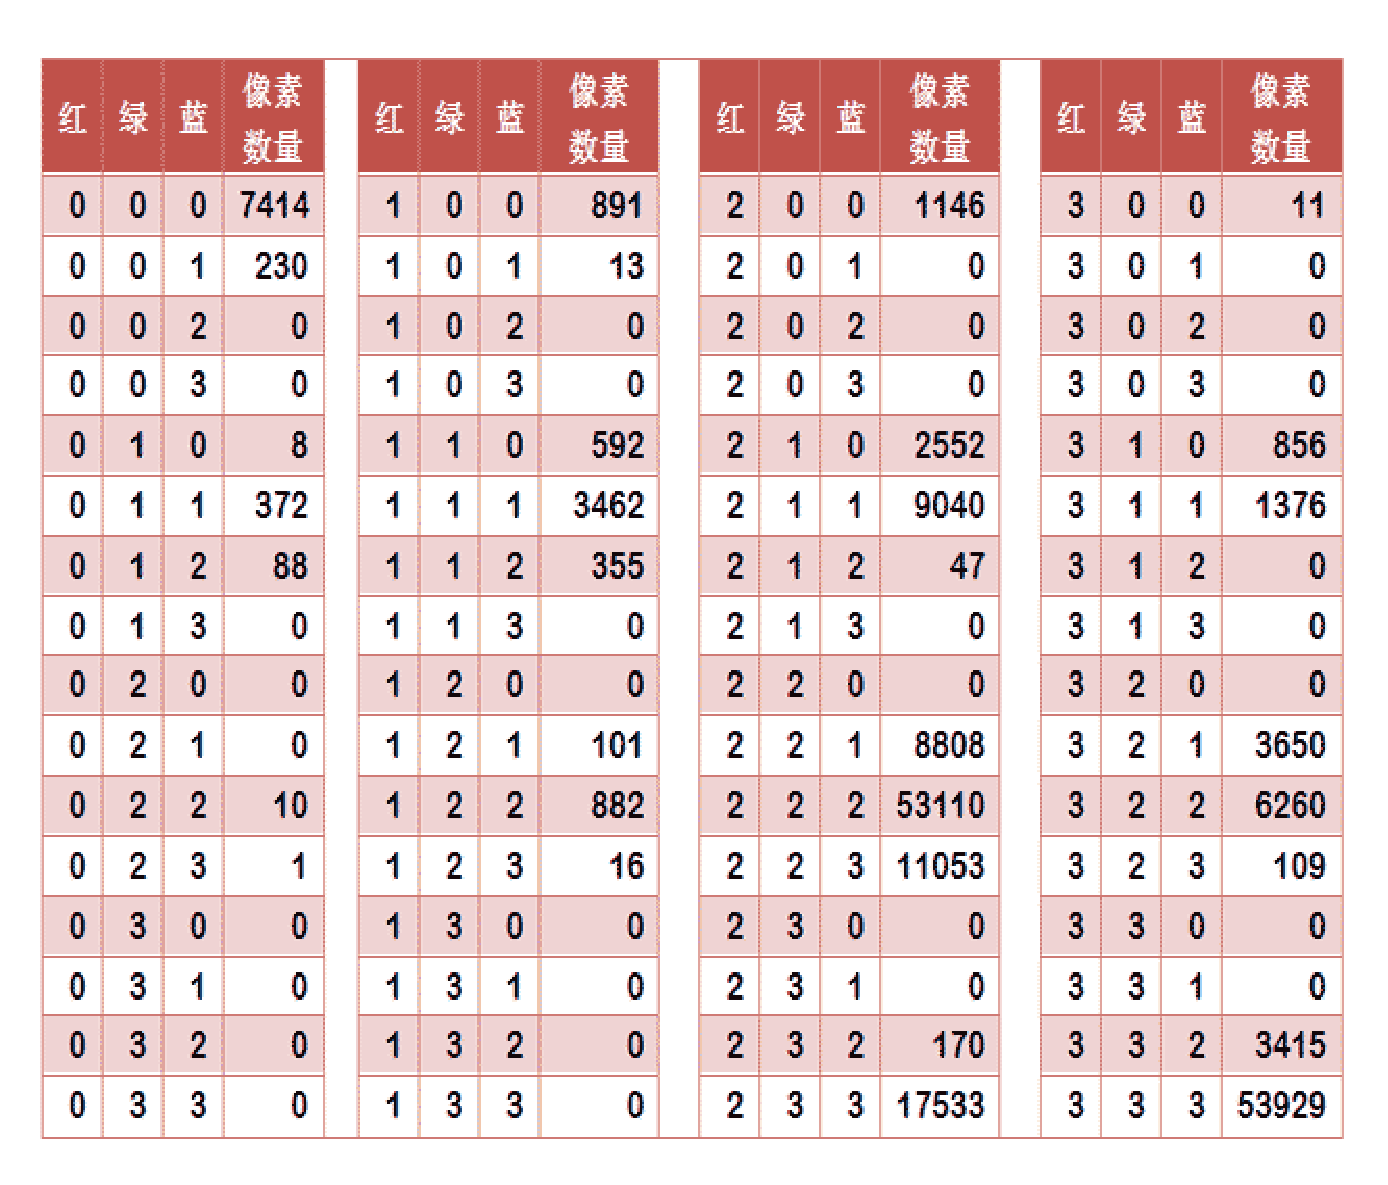
\includegraphics[width=0.95\textwidth]{figures/colordistribution.eps}
  \caption{颜色分布图}\label{fig:colordistribution}
\end{figure}

\section{大津阈值法}
图片处理中最常用的方法是将图片转换成较小的灰度图片,比如$50\times 50$,然后,再将灰度图片转成黑白图片(0-黑色,1-白色)。最终,使用0-1矩阵做相似性判断。在图片由灰度图片转换到黑白图片时,阈值选择是一个重要的步骤。

一般地,如果两张图片相似,那么它们的黑白轮廓自然也相近,一个合理的阈值应该能够正确呈现出图片的黑白轮廓,而反映轮廓清晰程度的重要因素是前景色与背景色的反差,反差越大则轮廓越明显。这就意味着,通过最小化前景色和背景色各自的类内差异(minimizing the intra-class variance),或者最大化类间差异(maximizing the inter-class variance)就可以找到理想的阈值$\theta$。

1979年,日本学者大津展之证明“类内差异最小”与“类间差异最大”是等价的,对应相同的阈值,这种通过最优化类内或类间差异,确定最佳阈值的简单方法就是大津阈值法(Otsu's thresholding method)。

假定一张图片共有$n$个像素,其中灰度值小于$\theta$的像素有$n_1$个,大于等于$\theta$的像素有$n_2$个,那么由此可以计算两种像素的权值$\omega_1 = n_1/n$和$\omega_2=n_2/n$。

再假定所有灰度值小于$\theta$的像素的平均值和方差分别为$\mu_1$和$\sigma_1$,所有灰度值大于等于阈值的像素的平均值和方差分别为$\mu_2$和$\sigma_2$,那么,可以计算类内差异和类间差异:
\begin{eqnarray}
  V_r &=& \omega_1\sigma_1^2 + \omega_2\sigma_2^2 \\
  V_e &=& \omega_1\omega_2(\sigma_1 - \sigma_2)^2
\end{eqnarray}
可以证明,两个等式是等价的,不过,从计算难度看,后者的计算要容易一些。

有了$50\times 50$像素的黑白缩略图,就等于有了一个$50\times 50$的0-1矩阵。矩阵的每个值对应原图的一个像素,0表示黑色,1表示白色。两个特征矩阵的不同之处越少,说明两张图片越相似。

\section{VisualRank}
在2008年北京国际万维网会议上,Google的两名科学家Yushi Jing和Shumeet Baluja介绍了一种图片搜索新型算法VisualRank,它通过直接分析图片内容,并充分利用图片名称、网络链接地址或者其他文本内容,寻找和排列图片。综合了图像识别、相似图像排序技术,应用到大规模图像搜索~\cite{jing2008visualrank}。

\chapter{基于评分的排名模型}
\section{牛顿冷却定律}
根据\textbf{牛顿冷却定律}(Newton's law of cooling)
\footnote{\href{http://www.ruanyifeng.com/blog/algorithm/}{阮一峰:算法与数学}},
“物体温度的变化速率正比例于物体同周围环境的温差”。%(The rate of change of the temperature of an object is proportional to the difference between its own temperature and the ambient temperature.)
假设在时刻$t$,物体温度是$T_t$,周围环境的温度不变,记为常量$T_{env}$,则冷却定律可以表示为微分形式
\begin{equation}
    T'_t = -\alpha(T_t-T_{env})
\end{equation}
其中,$\alpha>0$表示物体冷却系数。若以某个时点,如$t_0$为起始时刻,物体的初始温度为$T_0$,解微分方程可以得到物体温度随时间变化的规律
\begin{equation}
    T_t = T_{env} + (T_0 - T_{env})e^{-\alpha(t-t_0)}
\end{equation}

假设所有物体最终都会“冷寂”,环境温度等于0,就有
\begin{equation}
    T_t = T_0 e^{-\alpha(t-t_0)}
\end{equation}

对于新闻或博客,用户的点击、文章质量、文章发布距离现在的时间间隔(简称“年龄”)等属性是影响文章排名的重要因素。牛顿冷却定律(又称指数衰减规律)可以很好地体现时间对文章排名的影响:时间会降低文章的权重。系统首先为每篇文章赋予一个初始“温度”,随着文章年龄的增长,指数形式地降低文章的热度,其中冷却系数反映了物体温度变化的剧烈程度,如果希望文章热度变化缓慢,则可以选择比较小的$\alpha$,否则增大$\alpha$。

\section{HNRating}
2007年,创业孵化器Y Combinator的创始人Paul Graham
\footnote{Paul Graham,1964年生于英国,康奈尔大学本科、哈佛大学计算机科学博士,全球知名的程序员,风险投资专家,享有硅谷创业教父之美誉。1995年,他与麻省理工学院计算机教授Robert Morris 共同开发出世界上第一个互联网应用程序Viaweb,帮助个人用户在网上开店。1998年,Yahoo!公司以5,000万美元的价格收购Viaweb。
2005年他和Jessica Livingston(2008年两人结婚)联合创立Y Combinator孵化器。如今,YC 孵化器已经成为全球最出名的技术创业孵化器,已经成功孵化841家创业公司,包括Dropbox、Heroku、Airbnb、Bump、Justin.tv、Reddit、Disqus、Posterous 等明星公司,这些创业公司总计获得72亿美元的融资。}
创建Hacker News
\footnote{Hacker News: \href{http://thehackernews.com/}{http://thehackernews.com/}},
主要发布创业公司和骇客题材的社会化新闻。每条新闻(帖子)前都有一个上三角图形,如果用户觉得内容很好,可以点击一下,投上一票。系统根据得票数,会自动统计出热门新闻排行榜。但是,得票并非决定新闻排名的唯一因素,另外一个重要因素是时间,从而新闻要比旧闻获得更高的排名。系统新闻排序模型可以归结为用户投票与新闻年龄的函数,新闻的排名分值$S$可以表示为
\begin{equation}
   S = \frac{P-1}{(T+2)^G}
\end{equation}
其中,$P$是新闻的得票数目,减去1则忽略作者的投票。$T$是新闻发布距离现在的时间(以小时计)。$G$是重力因子(gravity),默认设置为1.8。重力因子越大,则旧帖子下沉的速度越快。

\section{Reddit热度评分}% Hot Rating
2005年6月,在接受 Y Combinator 的种子资金后,Alexis Ohanian 和 Steve Huffman 共同创立了 Reddit
\footnote{Reddit: \href{https://www.reddit.com/}{https://www.reddit.com/}}。
Reddit现已发展成为美国最火的社交新闻网站。2005年12月8日开始,Reddit社区用户可以评论帖子并投票:好评或差评,系统会根据得票数,更新“热贴排行榜”。

给定贴在发布时间$A$,可以计算距离Reddit评论功能开放时间点“$B=\text{2005年12月8日7:46:43}$”的间隔(以秒计)$t_s = A - B$,统计用户的投票结果,可以计算帖子好评数$U$与差评数$D$的差值$x=U-D$。Reddit根据帖子票差和年龄给帖子评分
\begin{equation}
    S = \log y + \frac{z t_s}{45000}
\end{equation}
其中,$y=\max\{|x|,1\},z=\sgn x$,对数函数取10为底。

分析评分公式的第一部分可以发现,帖子的得票票差越大(大多数用户观点一致),则帖子的得分越高,它不考虑投票的先后顺序影响。如果帖子富有争议,导致票差微小,则得分小于观点一致的帖子。假设两个同时发布的帖子,一个得分$U_1=10000,D_1=10001$,另一个得分$U_2=10,D_2=0$,前者得分为0,后者得分是1,整体来看,Reddit 推崇和谐社区建设,观点激进或少数派的帖子不太可能“榜上有名”。对于评分公式的第二部分,好评数大于差评数时,则新颖性会给帖子加分,反之,如果差评数高于好评数,那么新颖性会给帖子减分。目前,Reddit已经启用新的评论排名算法
\footnote{\href{http://jandan.net/2014/04/03/reddits-comment-sorting.html}{Reddit 的评论排序新算法}}。

\section{Reddit最佳评分}% Best Rating
基于用户投票进行排名的系统通常会犯两种类型的错误,使用“好评与差评的差值”或“好评率”对物品排名。第二种错误不是那么明显,假设用户对两个帖子的评价一个是$U_1=1, D_1=0$,一个帖子的评价是$U_2=95, D_1=5$,显然第一个帖子的好评率(100\%)大于第二个贴子(95\%)。从直观来看,根据好评率进行排序不合理。

假设每个用户的评价(好评或差评)都是一个独立随机事件,服从参数为$\hat{p}$的二项分布,好评率$p$是参数$\hat{p}$的一种估计。在统计学中,人们常使用置信区间估计真实参数的取值范围。使用相同的置信度$1-\alpha$,置信区间的宽度越小则表明参数估计越可信。比如,一个帖子有8个好评,2个差评,另一个帖子有80 个好评,20 个差评。两个帖子的好评率都是80\%,但是前者的置信区间是[70\%, 90\%],后者是[75\%, 85\%]。第二个置信区间比第一个置信区间窄,其置信区间的下限值更大,那么它的排名应该靠前。

对于大样本数据($np > 5,~~n(1 - p) > 5$),根据中心极限定理,二项分布的置信区间可以利用正态近似区间计算$\hat{p}\pm z\sqrt{\hat{p}(1-\hat{p})/n}$,在小样本数据上,其准确性较差。1927年,Edwin Wilson\cite{wilson1927probable}修正正态近似区间,提出Wilson区间公式
\begin{equation}
  \frac{1}{1 + z^2/n} \Big[\hat p + z^2/(2n) \pm z \sqrt{\hat p (1 - \hat p)/n + z^2/(4n^2)}~~\Big]
\end{equation}
用于处理小样本数据样本上的参数估计问题。$z$表示标准正态分布的$1-\frac{1}{2}\alpha$分位数,对于置信度$1-\alpha=0.95$,错误率为$\alpha=0.05$,则标准正态分布的$0.975$分位数等于$1.96$。Reddit使用\textbf{Wilson区间下界}给社区中的评论打分,下界越大评分越高
\begin{equation}
    S = \frac{1}{1 + z^2/n} \Big[~~\hat p + z^2/(2n) - z \sqrt{\hat p (1 - \hat p)/n + z^2/(4n^2)}~~\Big]
\end{equation}
如果选择分位数$1-\frac{1}{2}\alpha=0.975$,则有
\begin{equation}
    S = \frac{1}{1 + 3.8416/n} \Big[~~\hat p + 1.9208/n - 1.96 \sqrt{\hat p (1 - \hat p)/n + 0.9604/n^2}~~\Big]
\end{equation}

\section{Stack Overflow评分}
2008年,Jeff Atwood与Joel Spolsky创建了Stack Overflow
\footnote{Stack Overflow: \href{http://stackoverflow.com/}{http://stackoverflow.com/}},
目前是世界上最受欢迎的程序员问答社区。Stack Overflow 根据浏览量$n_v$,回答人数$m$,回答的质量评分$s_i,i=1,\ldots,m$,其他用户对问题好评与差评差值$e$,问题发布年龄$t_a = t-t_0$,最后一次更新时间$t_u = t-t_m$,对用户提交的问题评分:
\begin{equation}
    S = \frac{4 \log n_v + m e/5 +\sum\limits_i s_i}{\big[0.5(t_a + t_u + 2)\big]^{1.5}}
\end{equation}

\section{IDMb榜首250评分系统}
IMDb(Internet Movie Database)
\footnote{IMDb: \href{http://www.imdb.com.cn/}{http://www.imdb.com.cn/}}
是全球最大的一个电影资料库,包括几乎所有的电影及1982年以后的电视剧作。IMDb资料库包含影视作品、演员、电游资料及分级、评论数据,评分采用10分制,其使用的评分体系是目前最流行的电影评分系统。

IMDb根据真实贝叶斯估(true bayesian estimate)计算电影评分
\begin{equation}
    S = \frac{v}{v + m} \bar S + \frac{m}{v + m} C
\end{equation}
将排名前250的电影放到首页。电影的评分$S$是其基于当前数据库中所有电影的平均得分$\bar S$与平滑常量$C$(当前7.0)的加权平均,$v$表示电影当前的投票总数,$m$表示电影有资格进入前250榜单的最低得票数(当前25,000)。


\begin{shaded}
现代搜索引擎是一种检索互联网信息的应用程序,主要包括三个模块:采集信息、建立索引、检索信息。搜索引擎是传统信息检索的一个重要应用,它使用计算机程序(网络爬虫或蜘蛛)自动采集互联网数据,然后对采集到的信息进行合理组织与处理(去重、索引等),根据前台搜索界面接收到的用户检索需求,即时迅速地从采集数据中检索到相关文档,并按照相关程度由高到低以列表的形式反馈给用户。搜索引擎肇始于20世纪末的加拿大,经过20多年的迅猛发展,已经成为人们获取信息的一个重要手段。

1990年,加拿大McGill大学的Alan Emtage、Peter Deutsch与Bill Wheelan联合开发出的一种在线FTP文件索引工具\textbf{Archine},堪称世界首个搜索引擎。它汇集上百个计算机系统的FTP文件资源生成一个文件目录,用户可以使用Unix grep命令查询文件名,从而确定存储目标文件的计算机系统。1992年,Nevada大学的Steven Foster与Fred Barrie出于相同目的开发出\textbf{Veronica},用于搜索普通文本文件。1993年,Utah大学的Rhett Jones与Veronica目标同又开发出\textbf{Jughead}。Veronica与Jughead均受到Archine的影响,分别通过Archine Comic的两个经典漫画人物Veronica Lodge与Jughead Jones向Archine致敬,并且二者发送文件均是基于Gopher系统。

1993年6月,MIT大学的Matthew Gray期望能够追踪互联网发展速度,于是就创造出了世界上第一个网络爬虫程序万维网\textbf{Wanderer},更新以后爬虫程序能够获取真实的网址。爬虫程序每天访问同一个网页上百次,严重影响互联网的速度,人们开始质疑其用处。1993年10月,Martijn Koster开发出\textbf{ALIWEB}(Archie-Like Indexing of the Web)。ALIWEB只抓取少量网页元信息的,允许用户自己提交期望能被索引到的网页数据,如此可以节省大量的带宽资源。对于Wanderer,ALIWEB代表一种强有力的回应,遗憾的是许多人不知如何提交自己的网站。截至1993年12月,陆续又涌现出三个基于网络爬虫的搜索引擎:Scotland的\textbf{JumpStation}、Colorado大学Oliver McBryan的\textbf{万维网蠕虫}、NASA的\textbf{RBSE}(Repository-Based Software Engineering)爬虫。JumpStation采集网页的标题与头部信息,并使用简单的线性搜索执行检索。互联网数目的不断增长最终将JumpStation淘汰出局。万维网蠕虫对网页标题信息及URL建立索引,但是它与JumpStation一样,对检索到的网页一视同仁按照顺序进行排列。RSBE爬虫则实现了一个排序系统,但没有意识到链接分析或者网页内容缓存的重要性。如果用户无法提供确切名称,系统仍然难以找到目标文件。

1993年2月,斯坦福大学六名学生Graham Spencer、Joe Kraus、Mark Van Haren、Ryan Mc Intyre、Ben Lutch和Martin Reinfried成立Architext项目,意图利用字词间关系的统计分析提升搜索效率。1993年6月,他们发布了开发的搜索软件\textbf{Excite}用于网络搜索。1999年1月,@Home以65亿美元的价格收购Excite,并易名为Excite@Home。2001 年10月,Excite@Home破产,InfoSpace以1000万美元的价格将其买下。2002年5月,Excite停止使用自己的搜索引擎,改用元搜索引擎Dogpile。

1994年1月,世界上第一个提供分类目录和搜索功能的\textbf{EINet Galaxy}上线。1994年4月,斯坦福大学博士生Jerry Yang与David Filo共同创办\textbf{Yahoo!}用于收集它们喜欢的网页。随着收录数目与访问量的增加,Yahoo!开始支持简单的数据库搜索。由于Yahoo!收录的网页需要经过手工处理,算不上真正意义的搜索引擎。Yahoo! 陆续采用Altavista、Inktomi、Google提供的搜索引擎服务,推动了搜索引擎技术的发展。1994年4月20日,华盛顿大学的Brian Pinkerton发布
\textbf{WebCrawler},它是世界上第一个支持全文检索的搜索引擎。1994年7月20日,卡内基梅隆大学的Michael Mauldin研发的\textbf{Lycos}正式发布,它是搜索引擎发展史上的一次革命,不仅提供相关性排名,还支持前缀匹配与单词近似匹配,也是第一个在搜索结果页面中实现网页自动摘要,并且它的数据量远超其他搜索搜索引擎。1999年4月,Lycos改由Fast提供搜索引擎服务。1994年底,又一个重要的搜索引擎\textbf{Infoseek}发布。Infoseek友善的用户界面、大量附加服务使它声望日隆。而1995 年12月与Netscape 的战略性协议,使它成为一个强势搜索引擎:当用户点击Netscape浏览器上的搜索按钮时,弹出Infoseek的搜索服务,而此前由Yahoo! 提供该服务。2001 年2 月,Infoseek改用Overture的搜索结果。

1995年,华盛顿大学的Eric Selberg 和 Oren Etzioni开发出\textbf{MetaCrawler},成为世界首个元搜索引擎。元搜索引擎对用户的检索请求进行转换处理,按照格式要求提交给多个成员搜索引擎,最终将所有成员搜索引擎的搜索结果进行汇总并反馈给用户。1995年12月,\textbf{AltaVista}发布亮相,它推陈出新提供大量的创新服务,迅速成为搜索领域的一支新秀。它是第一个支持自然语言搜索、第一个支持高级搜索语法(如AND,OR,NOT 等)、并声称是第一个支持用户自主提交或删除网站网址,并保证24小时内可以检索到的搜索引擎。1995年9月26日,加州伯克利大学的Eric Brewer、Paul Gauthier联合创立\textbf{Inktomi}。1996年5月20 日,Inktomi公司正式成立,并发布新的搜索引擎\textbf{HotBot}。Inktomi公司声称HotBot每天抓取的网页数目超过1000万,远超其它搜索引擎。Hotbot成为随后几年最受欢迎的搜索引擎之一。

1998年9月4日,斯坦福大学的Larry Page与Sergey Brin联合成立\textbf{Google}公司。2004年8月19日,在纳斯达克上市。由于技术先进,经过短短十多年的发展,Google 已经成为全球最大的搜索引擎,搜索服务覆盖全球30多种语言、100多个国家。

1997年,挪威科技大学的Tor Egge成立FAST(Fast Search \& Transfer)公司,1999年5月发布搜索引擎\textbf{AllTheWeb}。FAST试图复制Inktomi的模式,向其他搜索引擎提供数据。它宣称在数据的新颖性、高级搜索功能、搜索结果聚类、本地化显示、图片搜索方面都比Google更具优势。2003年2月,FAST网络搜索部门被Overture 收购。2004年3月25日,Overture被Yahoo!收购。2011年4月4日,alltheweb.com网站重定向到Yahoo!搜索。

2000年,Rutgers大学的Apostolos Gerasoulis及其同事创立\textbf{Teoma},2001年春正式上线。2001年9月11日被Ask Jeeves以大约400万美元的价格收购,为ask.com提供搜索服务。Teoma排名算法ExpertRank比较独特,它同时基于主题分类、链接分析给网页排名。2000年,前Infoseek工程师Matt Wells创立\textbf{Gigablast},索引了2 亿多网页,向合作网站提供大规模高性能的实时信息检索服务。目前,Matt Wells是Gigablast唯一的维护人员,并于2013年7月将代码开源托管到GitHub。2000年5月16日,Yeogirl Yun创立\textbf{WiseNut},并于2001年9月正式上线。WiseNut引进一种新型数据库,并发明一种新技术WiseGuide实现对搜索结果自动聚类,但是对高级搜索、布尔查询、网页快照等功能它却视而不见。2002年4月,被分类目录提供商LookSmart以900万美元的价格收购,试图成为主流搜索引擎。

1997年10月29日,北京大学“网络与分布式系统”研究室研发的“\textbf{天网}”中英文搜索引擎系统正式在CERNET上提供服务。它是国家“九五”重点科技攻关项目“中文编码和分布式中英文信息发现”的研究成果,提供北京大学、中国科院等FTP站点的检索。2000年初,在国家973重点基础研究发展规划项目基金资助下成立“天网”搜索引擎课题组,继续为天网提供技术支持。1998年1月,\textbf{Openfind}创立,并由台湾中正大学吴升教授领导的GAIS实验室提供技术支持。Openfind是当时最好的中文搜索引擎,鼎盛时期同时为三大门户网站新浪、奇摩、雅虎提供中文搜索服务。2002年6月,Openfind重新发布基于GAIS30工程的Openfind搜索引擎Beta版,推出多元排名(PolyRank)算法,宣布累计抓取网页35亿,并踏入英文搜索领域。2000年1月18日,超链分析专利发明人、前Infoseek资深工程师李彦宏(Gigablast的创始人Matt Wells是其在Infoseek的同事)与UC Berkeley大学博士徐勇联合创立\textbf{百度}公司。2000 年6 月,百度正式推出独立搜索门户baidu.com,并开始为多个门户网站(如搜狐、新浪、雅虎中文等)提供搜索服务。2001年10月22日正式发布Baidu搜索引擎。2005 年,百度在美国纳斯达克上市,成为首家进入纳斯达克成分股的中国公司。百度提供了音乐、视频、图片、百科、文库等各种搜索服务,成为目前全球最大的中文搜索引擎。
\end{shaded}